% TODO: be careful about uniform classes, should be explicit and mentioned
% TODO: add paragraph on kernelization (and other techniques?)

\documentclass[a4paper,11pt,notitlepage]{report}

\usepackage{amsthm}
\usepackage{amsfonts}
\usepackage[british,english]{babel}
\usepackage[T1]{fontenc}
\usepackage[utf8]{inputenc}
\usepackage{listings, babel}
\usepackage{graphicx}
\lstset{breaklines=true,basicstyle=\ttfamily}
\usepackage[margin=2cm]{geometry}

\theoremstyle{plain}
\newtheorem{thm}{Theorem}[chapter] % reset theorem numbering for each chapter

\theoremstyle{definition}
\newtheorem{defn}[thm]{Definition} % definition numbers are dependent on theorem numbers
\newtheorem{exmp}[thm]{Example} % same for example numbers

\selectlanguage{english}
\title{report title}
\author{David Nilsson, davnils@kth.se \\ Advanced Individual Course In Computer
Science}

\begin{document}

\maketitle
\clearpage

\abstract{TODO}
\selectlanguage{english}

\tableofcontents

\chapter{Project Overview}
This is an overview of this project, including goals and how the report is outlined.

\section{Purpose}
The purpose of this project is divided into two parts.
TODO the first part
TODO the second part

\section{Method}
TODO: Describe how this report fits into the bigger picture, what else has been
done, and what the report contains.

\chapter{Parameterized Complexity Theory}
TODO: Brief intro to this chapter

\section{Motivation}
In classical complexity theory we are given a very general view of computation.
The asymptotic time and space complexity of problems is given as functions over the number of bits in the input.
This results in the classification of many problems as NP-hard (e.g. vertex cover, independent set), which is typically interpreted as the problem being difficult to solve.
Does exluding polynomial time algorithms for problems in general make them infeasible in practice?
For certain problems this might certainly be true but there is no fundamental reason to which this would hold in general.
Many problems have special cases that are easy to solve or approximation algorithms that are capable of finding decent solutions within polynomial time.
For example there might exist a polynomial time algorithm solving all cases when an aspect of the problem is considered constant, e.g. the number of vertices in a vertex cover.

Parameterized complexity theory aims to provide a theoretical foundation for asymptotic analysis on a more fine-grained scale.
This is achieved by not only considering inputs as a binary string but placing it into a context of the problem being solved.
All of this is achieved while still maintaining classical complexity classes and focusing on existing results.
This alternative view of complexity theory also forms natural ties with approximation algorithms, something which is studied in REF.

\section{Parameterized decision problems}
The first step in developing a more fine-grained theory is to describe how problems are expressed.
In addition to strings in the language $L$ to be decided, the following is also needed:

\begin{defn}
A \emph{parameterization} is a polynomial time computable function $k : \Sigma^* \rightarrow \mathbb{N}$
\end{defn}

A parameterized decision problem is given on the format: $(L, k)$ where $L \subseteq \Sigma^*$ and $k$ is a parameterization of $L$.
The following is the common parameterization of vertex cover, known as $p-VERTEX-COVER$:
\begin{itemize}
\item Input: Graph $G$, number of vertices in cover $s$
\item Parameterization: $k((G, s)) = s$.
\item Problem: Does $G$ have a vertex cover of size $\leq s$?.
\end{itemize}

In classical complexity theory, reductions are given between problems as polynomial time computable mappings between strings in the languages.
Naturally this notion does not extend trivially to parameterized problems since the parameterization must be handled as well.
This results in the following:

\begin{defn}
A reduction $R$ mapping strings between the two parameterized languages $(L, k)$ and $(L', k')$ satisfies:
\begin{itemize}
\item the reduction preserves membership, i.e $x \in L \Rightarrow R(x) \in L'$
\item $R(x)$ is computable in time $f(k(x)) * p(|x|)$ for any $x \in L$ where $f$ is a computable function and $p$ is a polynomial
\item there is some computable function $f(x) : \mathbb{N} \rightarrow \mathbb{N}$ s.t. $\forall x \in \Sigma^* : k'(x) < f(k(x))$
\end{itemize}
\end{defn}

Typically such a reduction is written as $L <^{fpt} L'$.
The specific runtime bound is common within parameterized complexity and will later play a crucial part when defining fixed parameter tractability.

The second constraint ensures that certain reductions are rejected as invalid reductions.
An example of this is considering vertex cover, using the parameterization in TODO, and extending this result to other graph problems.
Independent set is commonly related to vertex cover as having the size $|G| - |S|$ for a graph $G$ with vertex cover $S$ (TODO REF).
Does this imply that the decision version of independent set reduces to vertex cover under parameterized reductions, and hence also transferring hardness?
%TODO: complete argument (pro-tip: it doesn't hold!)

Furthermore, it is of interest to study if problems remain within some given set of languages when applied to some reduction $R$.

\begin{defn}
The \emph{closure} of a set $C$ of languages is defined as $\left[ C \right] = \left\{ L' : L \in C : L <^{fpt} L'\right\}$.
\end{defn}

\begin{defn}
%TODO: Verify this statement.
A set $C$ of languages is \emph{closed} if $\left[ C \right] = C$.
\end{defn}

\begin{defn}
The $n$'th slice of a parameterized problem $(L, k)$ is $\left\{ x \in L : k(x) = n \right\}$.
\end{defn}

An example of slices is $3-COLORABILITY$, which is the language formed by the slice where $n = 3$ when using the standard parameterization $p-COLORABILITY$.
Slices are used later on when relating parameterized complexity classes to classical ones but also when discussing hardness results.

\section{Fixed parameter tractability}
todo

\begin{defn}
%TODO: Verify this statement.
An fpt-algorithm $A(x, k)$ runs at most $f(k(x)) p(|x|)$ steps, for some computable function $f$ and a polynomial $p$.
\end{defn}

\begin{defn}
%TODO: Verify this statement.
The class $FPT$ consists of all languages decided by some fpt-algorithm.
\end{defn}

%TODO: Add FPT algorithm for vertex cover, thereby proving that p-VERTEX-COVER \in FPT.

There is a notable connection between languages in $FPT$ and the classical class $P$:

\begin{thm}
All slices of a language in $FPT$ are in $P$.
\end{thm}

By the contrapositive we have that if a slice $l'$ of a problem $L$, is not contained in $P$, it follows that the $L \not \in FPT$.
An example of this is the fact that $3-COLORABILITY$ is $NP$-hard, and hence if $P \not = NP$, it follows that $COLORABILITY \not \in FPT$.

\section{Relation to approximation}
todo

\section{Generalized classes}
todo

\section{Intermediate classes}
TODO: W[P], W-hierarchy (circuit definition), relate to existing classes

\section{Hardness results and lower bounds}
TODO: why? examples using p-CLIQUE, describe K-path result


\chapter{Counting Thin Subgraphs}
TODO: Brief intro to this chapter

\section{Introduction to counting patterns}
TODO: Graph isomorphism, \#k-path, Hamiltonian path (Björklund), counting trees, tree decompositions.
State of art results, some history.
Introduce the kaski paper.

\section{Tree decompositions and related measures}
TODO: tree decompositions (relate join trees), nice tree decompositions (all
critierias), labeling.
worst-case time-complexity and real-life resulsts for decompositions.
Dynprog over decompositions.

\section{Counting injective homomorphisms}
TODO: k-coloring (Diaz), subgraph isomorphism, injective homomorphisms (Fomin).

\section{Thin subgraphs as weighted disjoint triples}
TODO: Kaski construction

\begin{figure}[here]
\centering
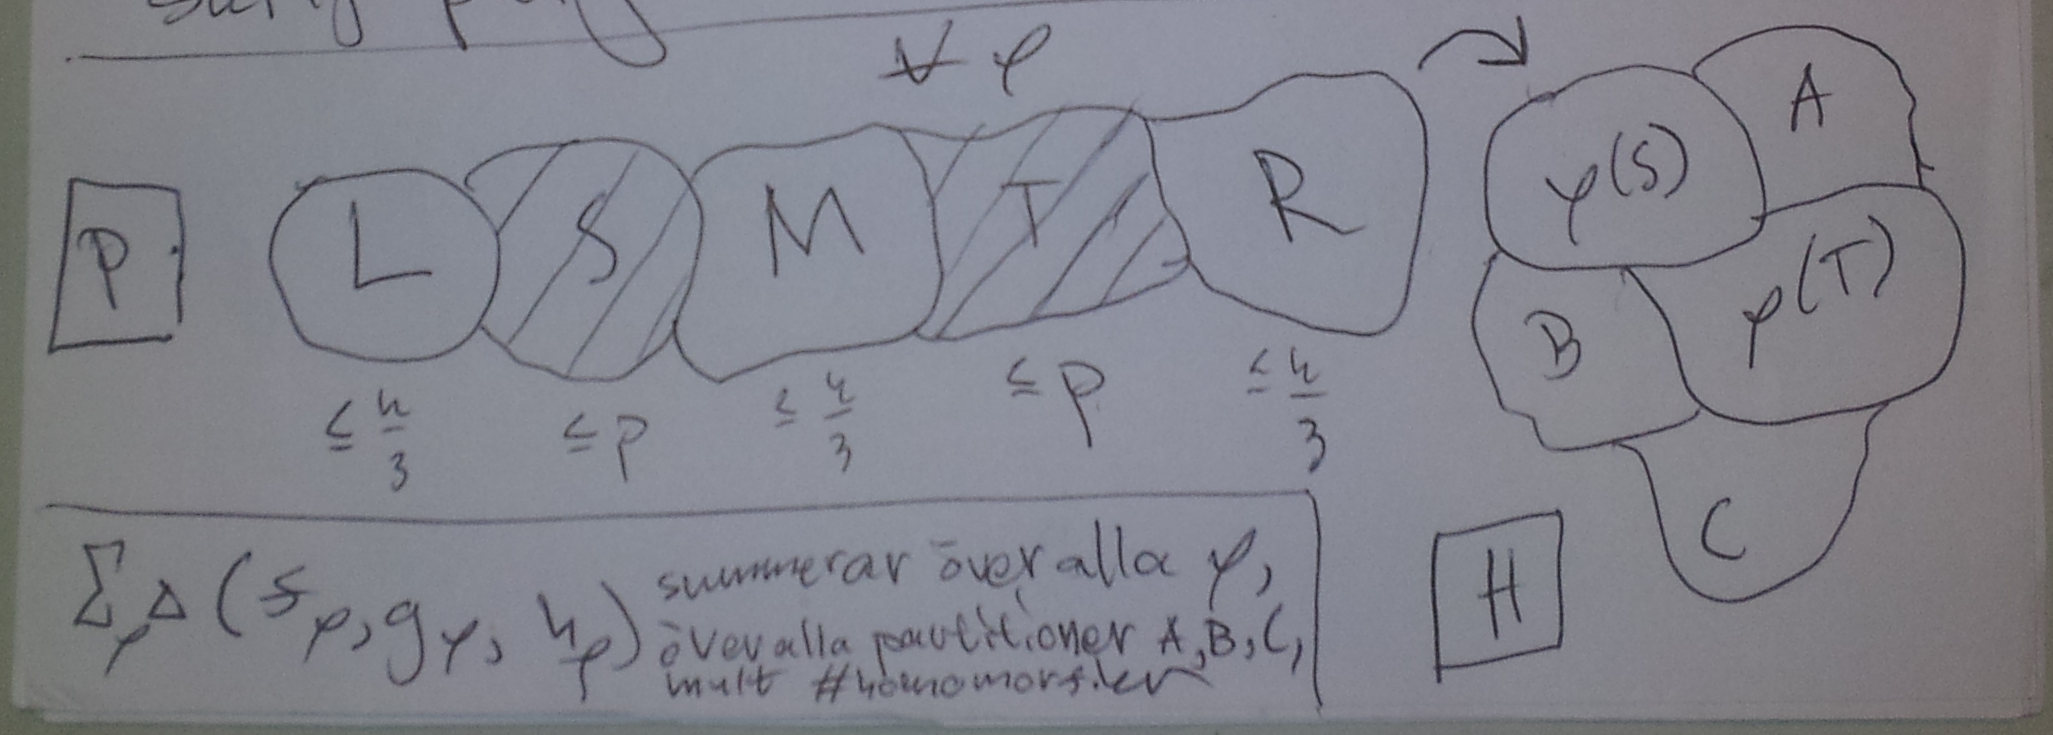
\includegraphics[width=10cm]{images/sketch_homo.png} 
\caption[todo]{todo}
\label{fig:homo-viz}
\end{figure}

\section{Efficient weighted disjoint triples}
TODO: Kaski construction


\chapter{Implementation}
TODO: Brief intro to this chapter

\section{General overview}
TODO: Describe implementation, trade-offs, correctness verification.

\section{Benchmarks}
TODO: Describe test data (generation and classes), scaling performance,
statistical assurance in resulsts, bottlenecks.

\section{Analysis}
TODO: analyze benchmarks

\chapter*{References}

tree-paper,
Diaz,
Fomin,
Kaski,
Björklund,
Flum-Grohe

\end{document}
